\documentclass[11pt, letterpaper]{memoir}
\usepackage{HomeworkStyle}

\begin{document}
	\begin{center}
		{\large	Quiz 12.1 -- Reaction Rates and Rate Equations}
	\end{center}
	{\large Name: \rule[-1mm]{4in}{.1pt} 
	
	\noindent
	For all questions in this quiz, consider the reaction: ~~ \ch{A + 2 B -> 3 C}. \\Below are graphs of the concentration of \ch{C} over time under three different initial conditions:
	
	\noindent \hspace{-2em} 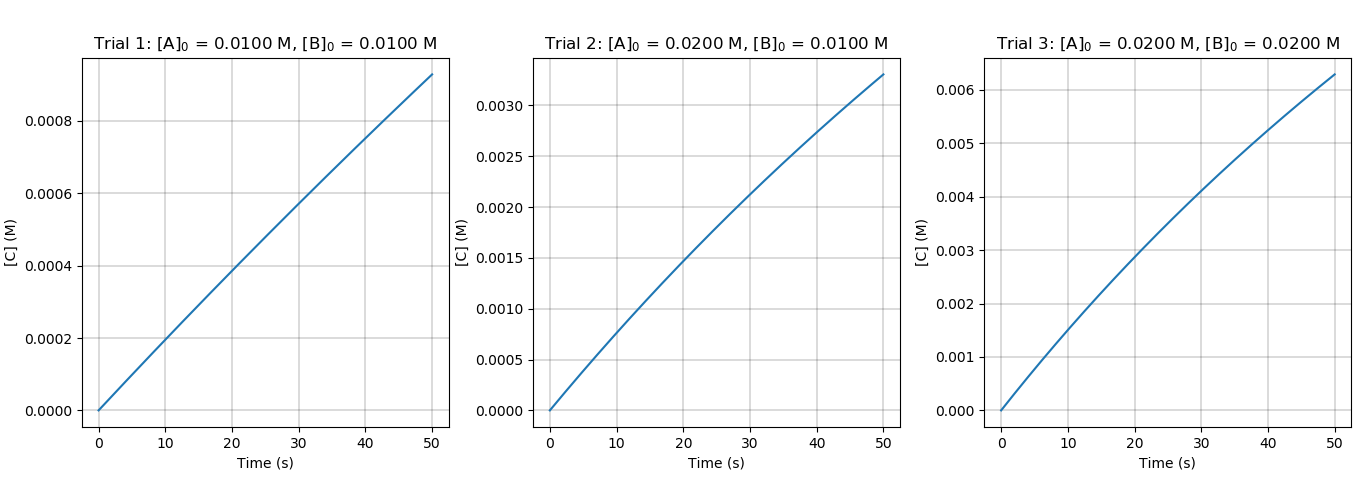
\includegraphics[width=1.1\linewidth]{Initial_Rates} 
	
	\subsection*{Question 1}
	From the data in the graphs, estimate the average reaction rate over the first $20~s$ for each trial
	
	\vspace{5em}
	\subsection*{Question 2}
	Find the reaction order for both of the reactants, and the overall reaction order
	
	\vspace{5em}
	\subsection*{Question 3}
	Give the value for the rate constant $k$, with appropriate units
	
	\vspace{5em}
	\subsection*{Question 4}
	Name the five factors which control rates of reaction:
	
	\newpage
	\newgeometry{margin=1.25in}
	\pagestyle{empty}
	\addtocounter{page}{-1}
	\section*{\emph{Ozymandius}}
	\paragraph{By Percy Bysshe Shelley}~
	\begin{verse}
		I met a traveller from an antique land,\\
		Who said—“Two vast and trunkless legs of stone\\
		Stand in the desert. . . . Near them, on the sand,\\
		Half sunk a shattered visage lies, whose frown,\\
		And wrinkled lip, and sneer of cold command,\\
		Tell that its sculptor well those passions read\\
		Which yet survive, stamped on these lifeless things,\\
		The hand that mocked them, and the heart that fed;\\
		And on the pedestal, these words appear:\\
		My name is Ozymandias, King of Kings;\\
		Look on my Works, ye Mighty, and despair!\\
		Nothing beside remains. Round the decay\\
		Of that colossal Wreck, boundless and bare\\
		The lone and level sands stretch far away.”
	\end{verse}
\end{document}
